\documentclass{esannV2}
\usepackage{graphicx}
\usepackage[latin1]{inputenc}
\usepackage{amssymb,amsmath,array}
\usepackage{subfigure}

%***********************************************************************
% !!!! IMPORTANT NOTICE ON TEXT MARGINS !!!!!
%***********************************************************************
%
% Please avoid using DVI2PDF or PS2PDF converters: some undesired
% shifting/scaling may occur when using these programs
% It is strongly recommended to use the DVIPS converters, and to submit
% PS file. You may submit a PDF file if and only if you use ADOBE ACROBAT
% to convert your PS file to PDF.
%
% Check that you have set the paper size to A4 (and NOT to letter) in your
% dvi2ps converter, in Adobe Acrobat if you use it, and in any printer driver
% that you could use.  You also have to disable the 'scale to fit paper' option
% of your printer driver.
%
% In any case, please check carefully that the final size of the top and
% bottom margins is 5.2 cm and of the left and right margins is 4.4 cm.
% It is your responsibility to verify this important requirement.  If these margin requirements and not fulfilled at the end of your file generation process, please use the following commands to correct them.  Otherwise, please do not modify these commands.
%
\voffset 0 cm \hoffset 0 cm \addtolength{\textwidth}{0cm}
\addtolength{\textheight}{0cm}\addtolength{\leftmargin}{0cm}

%***********************************************************************
% !!!! USE OF THE esannV2 LaTeX STYLE FILE !!!!!
%***********************************************************************
%
% Some commands are inserted in the following .tex example file.  Therefore to
% set up your ESANN submission, please use this file and modify it to insert
% your text, rather than staring from a blank .tex file.  In this way, you will
% have the commands inserted in the right place.

\begin{document}
%style file for ESANN manuscripts
\title{Deep Learning Vector Quantization}

%***********************************************************************
% AUTHORS INFORMATION AREA
%***********************************************************************
\author{Harm de Vries$^1$ and Second author$^2$
%
% Optional short acknowledgment: remove next line if non-needed
\thanks{This is an optional funding source acknowledgement.}
%
% DO NOT MODIFY THE FOLLOWING '\vspace' ARGUMENT
\vspace{.3cm}\\
%
% Addresses and institutions (remove "1- " in case of a single institution)
1- Universit\'{e} de Montr\'{e}al \\
\textit{mail@harmdevries.com}
%
% Remove the next three lines in case of a single institution
\vspace{.1cm}\\
2- School of Second Author - Dept of Second Author \\
Address of Second Author's school - Country of Second Author's school\\
}
%***********************************************************************
% END OF AUTHORS INFORMATION AREA
%***********************************************************************

\maketitle

\begin{abstract}
We introduce an extension of Generalized Learning Vector Quantization, a popular prototype based classifier, that incorporates non-linear metric learning by a deep neural network. The extra capacity 
\end{abstract}

\section{Introduction}

\section{Generalized Matrix Learning Vector Quantization}
We assume we are given training data $(\mathbf{x}^{(n)}, y^{(n)}) \in R^D \times \{0, ..., K-1\}$, $n=1, ..., N$, where $D$ is the dimensionality of the input, and $K$ the number of classes. A LVQ classifier consist of a set of prototypes ${\mathbf{w}_j} \in R^D, j=1, ..., M$ with an associated class label $c(w_j) \in \{1, ..., K\}$. In this work we consider one prototype per class, although it is straightforward to extend to multiple prototypes. Classification follows a nearest prototype scheme i.e. a new data point $\tilde{x}$ is assigned to the class of the nearest prototype $c(\mbox{arg min}_j d(\tilde{x}, \mathbf{w}_j))$ according to some distance measure $d(\tilde{x}, w_j)$. 

Training aims to find the locations of the prototypes such that the data points are assigned to their corresponding class labels. Generalized Learning Vector Quantization (GLVQ) \cite{sato1996generalized} aims to achieve this objective by minimizing the following training criterion:
\begin{equation}
 L_{GLVQ}(\theta) = \sum_n \phi(l^{(n)}) \mbox{~~with~~} l^{(n)} = \frac{d^{(n)}_+ - d^{(n)}_-}{d^{(n)}_+ + d^{(n)}_-}
\end{equation}
where $d^+ = \mbox{min}_{c(w_j) = y} d(x^{(n)}, \mathbf{w}_j)$ and $d^{(n)}_- = \mbox{min}_{c(\mathbf{w}_j)\neq y} d(x_i, \mathbf{w}_j)$ denote the distance to the closest correct and closest wrong prototype, respectively. The numerator denotes the margin between the correct and wrong class, while the denominator scales the term within the interval $[-1, 1]$. The scaling function $\phi$ provides a handle to balance error minimization and margin maximization. Using the step function corresponds to the non-differentiable zero-one loss, and using the identity function corresponds to an average margin maximization. A trade-off between the two terms can be realised by a scaling function $\phi(x) = \exp(\gamma x)$, where $\gamma > 0$ controls the steepness of the exponential. 

The main drawback of the GLVQ cost function is that it only displays correct training dynamics for correctly classified training examples\cite{sato1996generalized} i.e. when $l^{(n)} < 0$. To see this, note that for incorrectly classified examples the gradient with respect to the incorrect distance $4d^{(n)}_-/(d^{(n)}_+ - d^{(n)})^2$ is bigger than the gradient with respect to the correct class $\partial / \partial d^{(n)}_+ = 4d^{(n)}_+/(d^{(n)}_+ - d^{(n)})^2$. The repelling force on the prototypes then dominates the attractive force which leads to prototypes that diverge from the data distribution. One way to alleviate this problem is not to compare against the \emph{closest} incorrect prototype, but against the average distance to all incorrect prototypes. This smears out the repelling force over several prototypes, and makes it more likely that training dynamics are stable. In Supervised Neural Gas (SNG) \cite{SNG} this idea is realised by the following cost function\footnote{We note two reasonable alternatives: 1) the neighborhood function can be pushed into $l^{(n)}$ i.e. we define $d^{(n)}_- = \sum_{j \neq y^{(n)}} h_\tau(x^{(n)}, j) d(x^{(n)}, \mathbf{w}_j)$ and 2) the neighborhood function can also be replaced by a softargmin $h_\tau(x^{(n)}, j) = \exp(-\tau d(x, w_j)/\sum_k \exp(-\tau d(x^{(n)}, \mathbf{w}_k))$}:
\begin{equation}
 L_{SNG} = \sum_n \sum_{j\neq y^{(n)}} h_\tau \phi\left(\frac{d^{(n)}_+ - d(x^{(n)}, \mathbf{w}_j)}{d^{(n)}_+ + d(x^{(n)}, \mathbf{w}_j)}\right)
\end{equation}
Here, the neighborhood function $h_\tau(x^{(n)}, j) = \exp(-\tau k_j)/ \sum_{k=0}^{K-1} \exp(-\tau k)$ determines a (normalized) weight for each incorrect prototype loss that depends on its rank $k_j$, the number of prototypes for which are closer to the considered data point. Our training strategy is to start with small $\tau \rightarrow 0$, essentially replacing the minimum by an average over all incorrect prototypes, and slowly increase $\tau \rightarrow \infty$ such that we recover the GLVQ cost function. 

% There are two other important observation to make about the cost function: 
% \begin{itemize}
% \item The loss is invariant to the scale of the distances. That is, if each distance is multiplied by some constant $c \neq 0$\footnote{The closest correct and closest wrong prototype don't change}, the corresponding cost function value remains the same. 
% \item The loss is sensitive to an additive term. That is, if we add some constant $a > 0$ to the distances $d^+$ and $d^-$, this contribution will cancel in the numerator while it will add $2a$ to the denominator. For correctly classified data points (i.e. negative terms) this will increase the cost function value.          
% \end{itemize} 
% In summary, the first bullet point points out that we are maximizing a \emph{scale-invariant} margin. The second point is important to provide low confidence values far away from the data as will be explained in the next section. 

\section{Deep GLVQ}
We propose to extend the GLVQ cost function by parameterizing the distance function as:
\begin{equation}
 d(x, w_j) = \|f(\mathbf{x}; \theta) - \mathbf{w}_j\|^2_2
\end{equation}
where $f$ is a deep neural network with parameters $\mathbf{\theta}$. Usually, the prototypes live in the input space, but here we decide to let them live in the embedding space. It saves computational time because we don't have to do a forward and backward pass through the neural network $f$ for the prototypes. In addition, the embedding space is often much smaller than the input space, hence the prototype parameters take less memory in the embedding space. 

Although prototypes are often considered as class conditional examplars,  

\section{Related work}
The last layer in a deep neural network is frequently a softmax\footnote{Better characterised by softargmax}:
\begin{equation}
p(\hat{y}_j| \mathbf{x}^{(n)}) = \frac{\exp(w_j^\top \mathbf{x} + b_i)}{\sum_i \exp(w_i^\top \mathbf{x} + b_i)}
\end{equation}
which provides a distribution over the output labels. It is followed by a cross entropy loss $L_{cross-entropy} = \sum_{k=1}^K p(y_k|\mathbf{x}) \ln p(\hat{y}_k|\mathbf{x})$ which compares the conditional output distribution against the target distribution $p(\mathbf{y}|\mathbf{x})$. For crisp classification problems the target distribution is a $1-$of$-K$ vector, and the loss function simplifies to the negative log likelihood (NLL):
\begin{equation}
 - \sum_{n=1}^N \ln p(\hat{y}^{(n)}_j|\mathbf{x}^{(n)})
\end{equation}

To illustrate the difference with GLVQ, we provide an artifically generated three-class problem as shown in Fig. \ref{figure:diff_glvq_softmax}. 

\begin{figure}[t]
\centering{
\subfigure[Softmax]{
 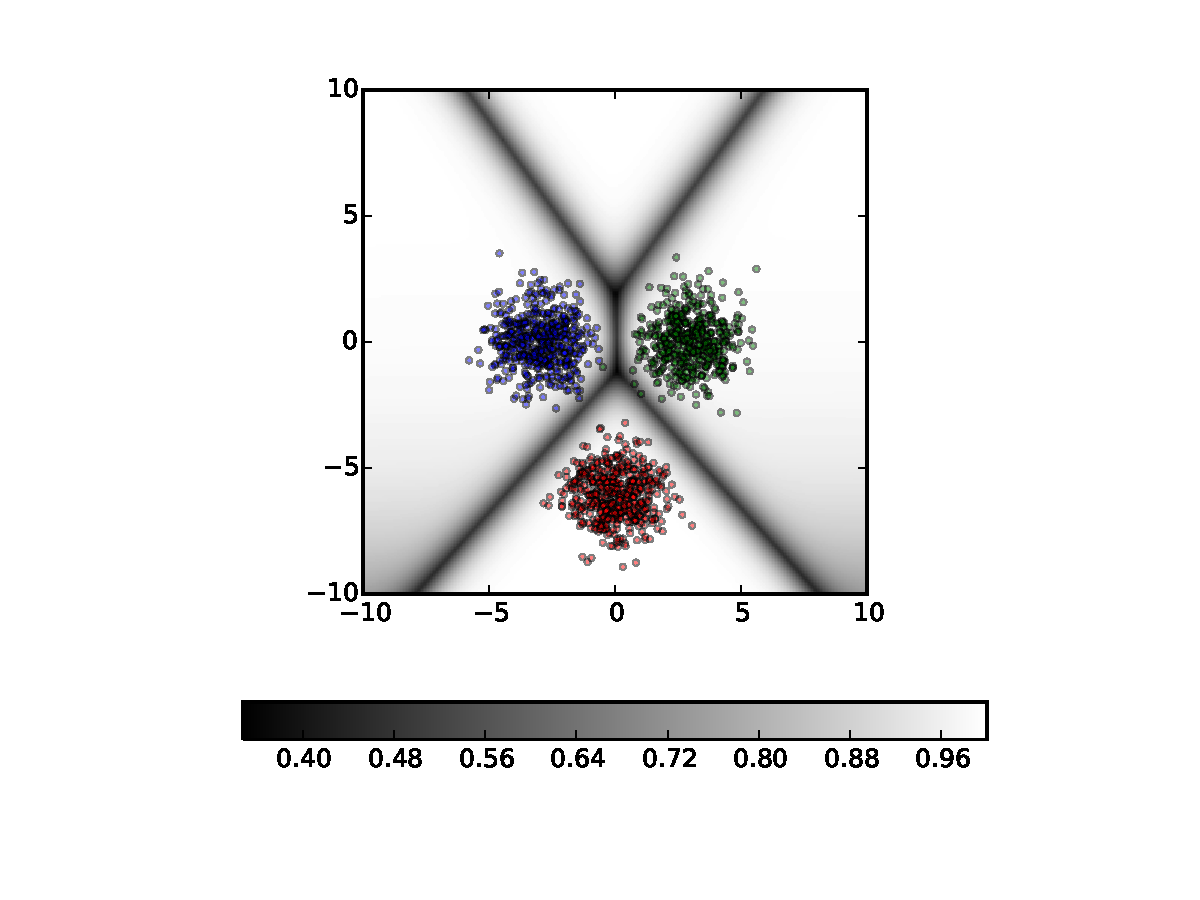
\includegraphics[width=0.48\textwidth, trim={3cm 0 1cm 0}]{../mnist/figures/softmax.pdf}}
\subfigure[GLVQ]{
 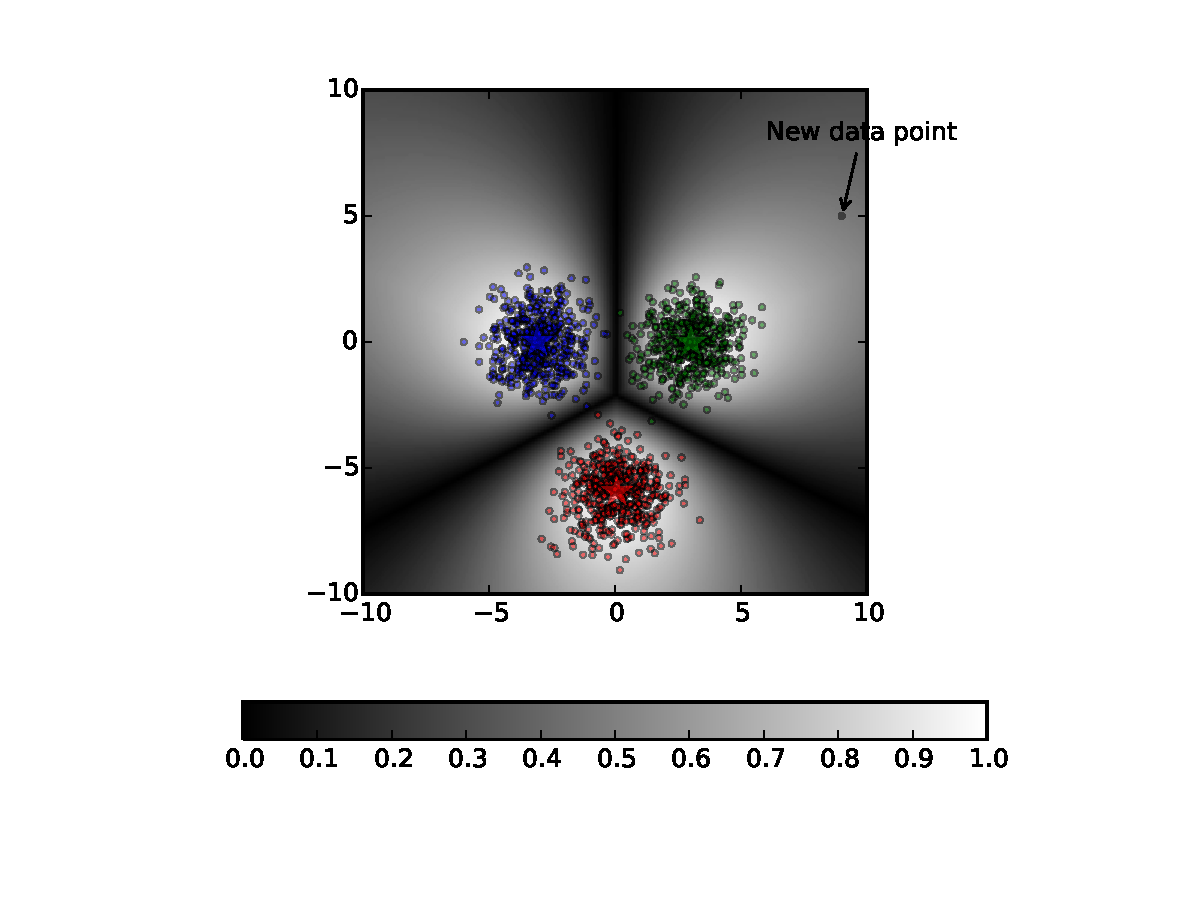
\includegraphics[width=0.48\textwidth, trim={3cm 0 1cm 0}]{../mnist/figures/lvq.pdf}}}
\caption{An artifically generated three class problem for which we have trained (a) a softmax classifier and (b) a GLVQ classifier. The background color (white for high) indicates the confidence values for a decision, that is $\mbox{arg max}_i\ p(y_j|x)$ for the softmax and $-\frac{d^{+} - d^{-}}{d^{+} + d^{-}}$\protect\footnotemark for the GLVQ classifier. The softmax classifier will assign a high confidence value to new data point in the right upper corner (far from the data), while GLVQ will not. }
\label{figure:diff_glvq_softmax}
\end{figure}

\footnotetext{We multiplied the cost with $-1$ such that higher values indicates higher confidence.}


\section{Experiments}
\subsection{MNIST}
We use a fully connected neural network with $1200-1200-100$ hidden units, followed by either a log softmax or GLVQ. All units have rectified linear activations. The networks are trained with batch normalization \cite{DBLP:journals/corr/IoffeS15}, and additive gaussian noise of standard deviation $0.5$ on the inputs. 

\subsubsection{Adversarial examples}
We illustrate the confidence values for 

\begin{figure}[ht]
\centering{
\subfigure[Softmax]{
 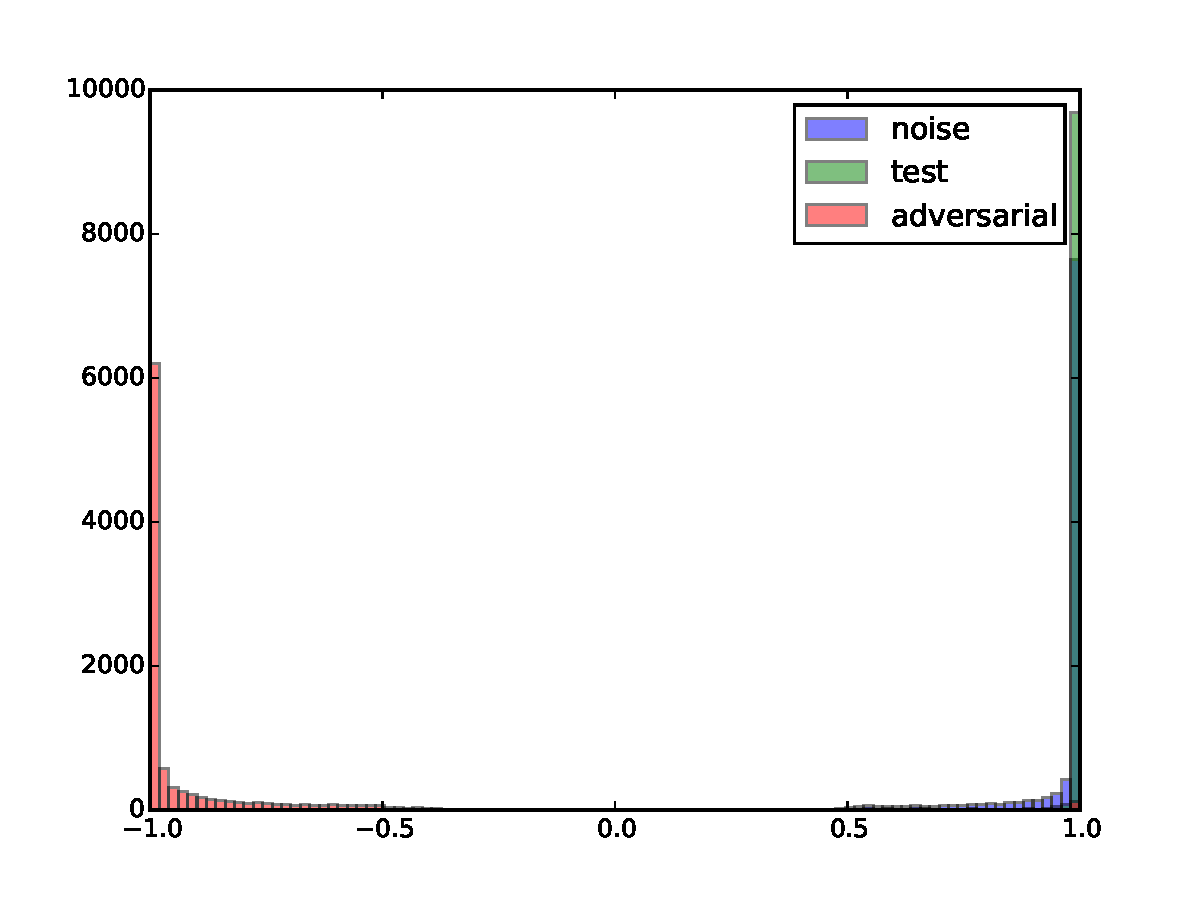
\includegraphics[width=0.48\textwidth]{../mnist/figures/softmax_conf.pdf}}
\subfigure[GLVQ]{
 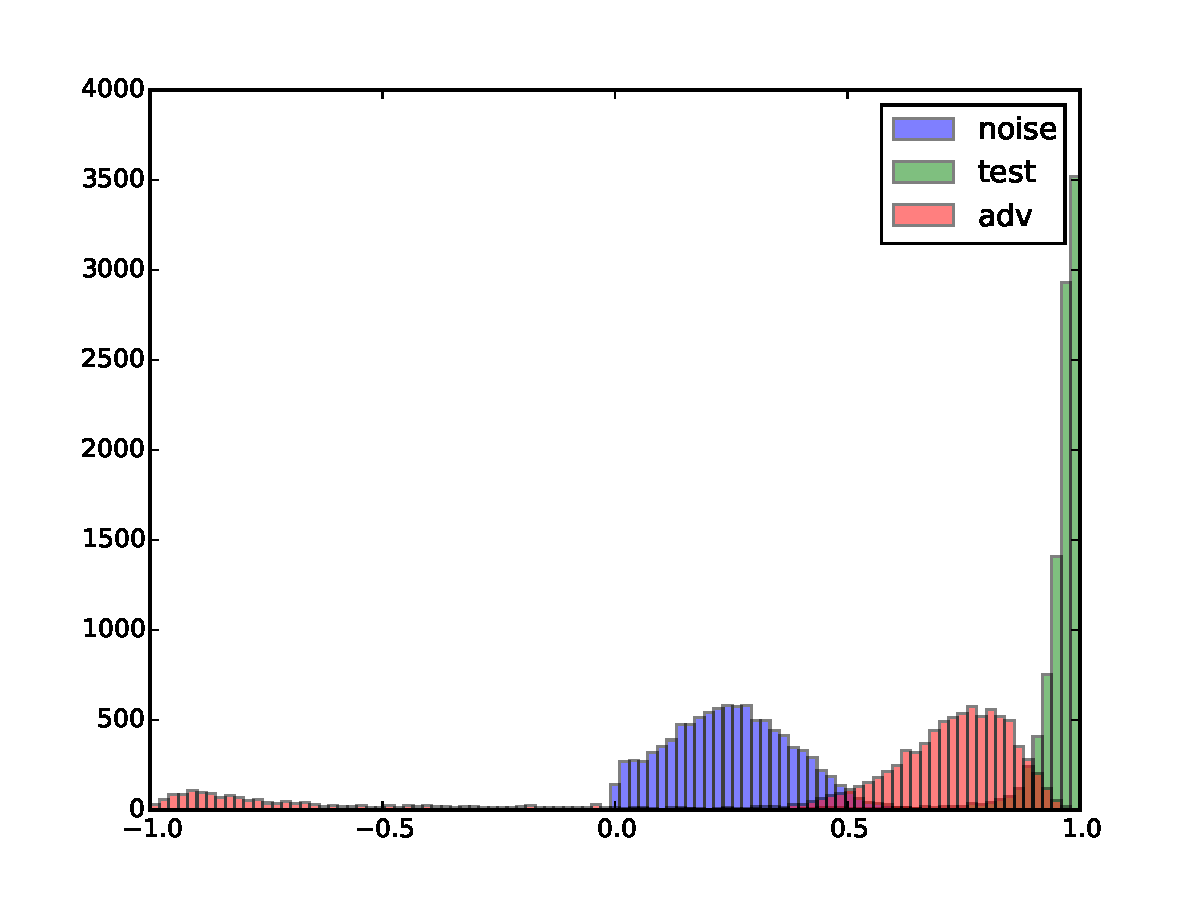
\includegraphics[width=0.48\textwidth]{../mnist/figures/lvq_conf.pdf}}}
\caption{Histogram of the confidence values for the neural network trained with a) softmax and b) GLVQ on MNIST. The green bars indicate the confidence values for the test set, the blue bars indicate the confidence values for noise drawn from $\mathcal{U}(0.0, 1.0)^{784}$ and the red bars denote the confidence for adversarial examples on the test set.}
\end{figure}

\subsection{CIFAR10}


\section{Conclusion}
% ****************************************************************************
% BIBLIOGRAPHY AREA
% ****************************************************************************

\begin{footnotesize}

% IF YOU USE BIBTEX,
% - DELETE THE TEXT BETWEEN THE TWO ABOVE DASHED LINES
% - UNCOMMENT THE NEXT TWO LINES AND REPLACE 'Name_Of_Your_BibFile'

\bibliographystyle{unsrt}
\bibliography{refs}

\end{footnotesize}

% ****************************************************************************
% END OF BIBLIOGRAPHY AREA
% ****************************************************************************
\appendix
\section{Softmax follows from gaussian class-conditionals}
Let's assume that the class-conditional distribution $p(x|y_j) = \frac{1}{Z} \exp(-\frac{1}{2\sigma^2}(\mathbf{x} - \mathbf{w}_j)^{\top}(\mathbf{x} - \mathbf{w}_j))$ is an isotropic Gaussian distribution with normalization constant $Z = ..$. 

\end{document}